% Options for packages loaded elsewhere
\PassOptionsToPackage{unicode}{hyperref}
\PassOptionsToPackage{hyphens}{url}
\PassOptionsToPackage{dvipsnames,svgnames,x11names}{xcolor}
%
\documentclass[
  man,floatsintext]{apa7}
\usepackage{amsmath,amssymb}
\usepackage{lmodern}
\usepackage{iftex}
\ifPDFTeX
  \usepackage[T1]{fontenc}
  \usepackage[utf8]{inputenc}
  \usepackage{textcomp} % provide euro and other symbols
\else % if luatex or xetex
  \usepackage{unicode-math}
  \defaultfontfeatures{Scale=MatchLowercase}
  \defaultfontfeatures[\rmfamily]{Ligatures=TeX,Scale=1}
\fi
% Use upquote if available, for straight quotes in verbatim environments
\IfFileExists{upquote.sty}{\usepackage{upquote}}{}
\IfFileExists{microtype.sty}{% use microtype if available
  \usepackage[]{microtype}
  \UseMicrotypeSet[protrusion]{basicmath} % disable protrusion for tt fonts
}{}
\makeatletter
\@ifundefined{KOMAClassName}{% if non-KOMA class
  \IfFileExists{parskip.sty}{%
    \usepackage{parskip}
  }{% else
    \setlength{\parindent}{0pt}
    \setlength{\parskip}{6pt plus 2pt minus 1pt}}
}{% if KOMA class
  \KOMAoptions{parskip=half}}
\makeatother
\usepackage{xcolor}
\IfFileExists{xurl.sty}{\usepackage{xurl}}{} % add URL line breaks if available
\IfFileExists{bookmark.sty}{\usepackage{bookmark}}{\usepackage{hyperref}}
\hypersetup{
  pdftitle={An analysis on Safety and Impact on the Job Market caused by Automation},
  pdfauthor={Rushabh Hitesh Barbhaya1},
  pdflang={en-EN},
  pdfkeywords={Automation, Jobs, Aviation, Self Driving Cars, Engineering, Science, Production, Safety, Lifestyle},
  colorlinks=true,
  linkcolor={blue},
  filecolor={Maroon},
  citecolor={Blue},
  urlcolor={Blue},
  pdfcreator={LaTeX via pandoc}}
\urlstyle{same} % disable monospaced font for URLs
\usepackage{graphicx}
\makeatletter
\def\maxwidth{\ifdim\Gin@nat@width>\linewidth\linewidth\else\Gin@nat@width\fi}
\def\maxheight{\ifdim\Gin@nat@height>\textheight\textheight\else\Gin@nat@height\fi}
\makeatother
% Scale images if necessary, so that they will not overflow the page
% margins by default, and it is still possible to overwrite the defaults
% using explicit options in \includegraphics[width, height, ...]{}
\setkeys{Gin}{width=\maxwidth,height=\maxheight,keepaspectratio}
% Set default figure placement to htbp
\makeatletter
\def\fps@figure{htbp}
\makeatother
\setlength{\emergencystretch}{3em} % prevent overfull lines
\providecommand{\tightlist}{%
  \setlength{\itemsep}{0pt}\setlength{\parskip}{0pt}}
\setcounter{secnumdepth}{-\maxdimen} % remove section numbering
% Make \paragraph and \subparagraph free-standing
\ifx\paragraph\undefined\else
  \let\oldparagraph\paragraph
  \renewcommand{\paragraph}[1]{\oldparagraph{#1}\mbox{}}
\fi
\ifx\subparagraph\undefined\else
  \let\oldsubparagraph\subparagraph
  \renewcommand{\subparagraph}[1]{\oldsubparagraph{#1}\mbox{}}
\fi
\newlength{\cslhangindent}
\setlength{\cslhangindent}{1.5em}
\newlength{\csllabelwidth}
\setlength{\csllabelwidth}{3em}
\newlength{\cslentryspacingunit} % times entry-spacing
\setlength{\cslentryspacingunit}{\parskip}
\newenvironment{CSLReferences}[2] % #1 hanging-ident, #2 entry spacing
 {% don't indent paragraphs
  \setlength{\parindent}{0pt}
  % turn on hanging indent if param 1 is 1
  \ifodd #1
  \let\oldpar\par
  \def\par{\hangindent=\cslhangindent\oldpar}
  \fi
  % set entry spacing
  \setlength{\parskip}{#2\cslentryspacingunit}
 }%
 {}
\usepackage{calc}
\newcommand{\CSLBlock}[1]{#1\hfill\break}
\newcommand{\CSLLeftMargin}[1]{\parbox[t]{\csllabelwidth}{#1}}
\newcommand{\CSLRightInline}[1]{\parbox[t]{\linewidth - \csllabelwidth}{#1}\break}
\newcommand{\CSLIndent}[1]{\hspace{\cslhangindent}#1}
\ifLuaTeX
\usepackage[bidi=basic]{babel}
\else
\usepackage[bidi=default]{babel}
\fi
\babelprovide[main,import]{english}
% get rid of language-specific shorthands (see #6817):
\let\LanguageShortHands\languageshorthands
\def\languageshorthands#1{}
% Manuscript styling
\usepackage{upgreek}
\captionsetup{font=singlespacing,justification=justified}

% Table formatting
\usepackage{longtable}
\usepackage{lscape}
% \usepackage[counterclockwise]{rotating}   % Landscape page setup for large tables
\usepackage{multirow}		% Table styling
\usepackage{tabularx}		% Control Column width
\usepackage[flushleft]{threeparttable}	% Allows for three part tables with a specified notes section
\usepackage{threeparttablex}            % Lets threeparttable work with longtable

% Create new environments so endfloat can handle them
% \newenvironment{ltable}
%   {\begin{landscape}\centering\begin{threeparttable}}
%   {\end{threeparttable}\end{landscape}}
\newenvironment{lltable}{\begin{landscape}\centering\begin{ThreePartTable}}{\end{ThreePartTable}\end{landscape}}

% Enables adjusting longtable caption width to table width
% Solution found at http://golatex.de/longtable-mit-caption-so-breit-wie-die-tabelle-t15767.html
\makeatletter
\newcommand\LastLTentrywidth{1em}
\newlength\longtablewidth
\setlength{\longtablewidth}{1in}
\newcommand{\getlongtablewidth}{\begingroup \ifcsname LT@\roman{LT@tables}\endcsname \global\longtablewidth=0pt \renewcommand{\LT@entry}[2]{\global\advance\longtablewidth by ##2\relax\gdef\LastLTentrywidth{##2}}\@nameuse{LT@\roman{LT@tables}} \fi \endgroup}

% \setlength{\parindent}{0.5in}
% \setlength{\parskip}{0pt plus 0pt minus 0pt}

% Overwrite redefinition of paragraph and subparagraph by the default LaTeX template
% See https://github.com/crsh/papaja/issues/292
\makeatletter
\renewcommand{\paragraph}{\@startsection{paragraph}{4}{\parindent}%
  {0\baselineskip \@plus 0.2ex \@minus 0.2ex}%
  {-1em}%
  {\normalfont\normalsize\bfseries\itshape\typesectitle}}

\renewcommand{\subparagraph}[1]{\@startsection{subparagraph}{5}{1em}%
  {0\baselineskip \@plus 0.2ex \@minus 0.2ex}%
  {-\z@\relax}%
  {\normalfont\normalsize\itshape\hspace{\parindent}{#1}\textit{\addperi}}{\relax}}
\makeatother

% \usepackage{etoolbox}
\makeatletter
\patchcmd{\HyOrg@maketitle}
  {\section{\normalfont\normalsize\abstractname}}
  {\section*{\normalfont\normalsize\abstractname}}
  {}{\typeout{Failed to patch abstract.}}
\patchcmd{\HyOrg@maketitle}
  {\section{\protect\normalfont{\@title}}}
  {\section*{\protect\normalfont{\@title}}}
  {}{\typeout{Failed to patch title.}}
\makeatother

\usepackage{xpatch}
\makeatletter
\xapptocmd\appendix
  {\xapptocmd\section
    {\addcontentsline{toc}{section}{\appendixname\ifoneappendix\else~\theappendix\fi\\: #1}}
    {}{\InnerPatchFailed}%
  }
{}{\PatchFailed}
\keywords{Automation, Jobs, Aviation, Self Driving Cars, Engineering, Science, Production, Safety, Lifestyle\newline\indent Word count: 3,484}
\usepackage{lineno}

\linenumbers
\usepackage{csquotes}
\usepackage[titles]{tocloft}
\cftpagenumbersoff{figure}
\renewcommand{\cftfigpresnum}{\itshape\figurename\enspace}
\renewcommand{\cftfigaftersnum}{.\space}
\setlength{\cftfigindent}{0pt}
\setlength{\cftafterloftitleskip}{0pt}
\settowidth{\cftfignumwidth}{Figure 10.\qquad}
\cftpagenumbersoff{table}
\renewcommand{\cfttabpresnum}{\itshape\tablename\enspace}
\renewcommand{\cfttabaftersnum}{.\space}
\setlength{\cfttabindent}{0pt}
\setlength{\cftafterloftitleskip}{0pt}
\settowidth{\cfttabnumwidth}{Table 10.\qquad}
\makeatletter
\renewcommand{\paragraph}{\@startsection{paragraph}{4}{\parindent}%
  {0\baselineskip \@plus 0.2ex \@minus 0.2ex}%
  {-1em}%
  {\normalfont\normalsize\bfseries\typesectitle}}

\renewcommand{\subparagraph}[1]{\@startsection{subparagraph}{5}{1em}%
  {0\baselineskip \@plus 0.2ex \@minus 0.2ex}%
  {-\z@\relax}%
  {\normalfont\normalsize\bfseries\itshape\hspace{\parindent}{#1}\textit{\addperi}}{\relax}}
\makeatother

\ifLuaTeX
  \usepackage{selnolig}  % disable illegal ligatures
\fi

\title{An analysis on Safety and Impact on the Job Market caused by Automation}
\author{Rushabh Hitesh Barbhaya\textsuperscript{1}}
\date{}


\shorttitle{Safety and Jobs in Automated World}

\authornote{

This paper is for the Harrisburg University of Science and Technology's graduate course of Analytics GRAD 695 \& ANLY 699. This paper uses actual research for analysis. All the research done by this paper can is reproducible. This document not peer reviewed and peer tested and is therefore for internal use of Harrisburg University of Science and Technology. This research should not be used as a reference in professional study and research.

Correspondence concerning this article should be addressed to Rushabh Hitesh Barbhaya, 326 Market St, Harrisburg, PA 17101. E-mail: \href{mailto:RBarbhaya@my.harrisburgu.edu}{\nolinkurl{RBarbhaya@my.harrisburgu.edu}}

}

\affiliation{\vspace{0.5cm}\textsuperscript{1} Harrisburg University of Science and Technology}

\abstract{%
PlaceHolder
}



\begin{document}
\maketitle

Artificial Intelligence, Machine Learning, Robots, Automation usually outline the news as the cause for mass layoffs, for example, as observed by Mackie (2021). McClure (2018) has similarly observed a correlation between the rise of mainstay automated solutions and growing health and safety concerns. The concern for technology replacing jobs has been known and documented since the 16th century. Hills (1989) and Fleming (2020) notes observe that, in 1589, William Lee's invention of the machine that made stockings had caused a riot in the country. The book ``The Luddites; Machine-Breaking in Regency England,'' authored by Thomis (1972) published in 1972, notes the rise of Luddism. Luddism is a working-class movement asking technology to work with employees and not against them. A modern scripture, ``The Digital Divide'' by Nie and Erbring (2001), has a unique perspective on this. The digital divide refers to the rift caused by a lack of access to information across gender, race, and age, among other demographic keys. Nie and Erbring (2001) observe that the gap is narrowing in current times. Robinson et al. (2003) pushes findings by Nie and Erbring (2001) a bit further and notices the information's bias. However, they do not account for future and future technology.

An article by Smith (2019) states that 50\% of Americans believe that Robots will replace innumerable jobs across the industry. The critical point is that 80\% believe that their jobs will be secure. It seems counterintuitive, but humans always find a more specialized role, which is not surprising. Acemoglu and Autor (2011) outlines the same observations. They observed a decline in low-skilled jobs, raising differences between each level of workers. Acemoglu and Autor (2011) observe that computers replace jobs where cognitive skills and manual input are obligatory. The author did not break down the observations across different industrial sectors where the writer will be observing the results. Authors also published another article Autor et al. (2003), noting an increased skill level of an employee in computer-intense industries. This time the author only focused on technology-focused industries and missed out on observing the same trend across other industrial sectors, which is the focus of this research. Humans also fear ``being left behind,'' says Song (2003), and will always try to cover the skills they offset. Illustrated by other papers in this article, we observe a decline in low-skill jobs that are labor-intensive jobs.

\hypertarget{automation-in-varioius-industires}{%
\section{Automation in varioius industires}\label{automation-in-varioius-industires}}

Abernathy and Townsend (1975) observes the evolution of manual processes. A process that starts as simple logic; evolves into a complex one over time. This evolution in process generates inefficiencies. Machines are employed to bring back the lost inefficiencies in the system. The author did not account for how these trends are observed in different industrial sectors. Evangelista and Vezzani (2012) balances out the corporate perspective and speaks for human evolution. As robots take on menial jobs, humans find a more specialized roles. Those specialized roles spikes growth and knowledge. Similarly, Bainbridge (1982) describes how automation can work in tandem with humans. Humans can take more managerial roles and let machines handle the rule-based task.

\hypertarget{aviation}{%
\subsection{Aviation}\label{aviation}}

At the time of writing, the airline industry is almost automated. Auto-pilot, take-off and landing assistance, navigation, and other critical functions are automated. However, we still see pilots in the cockpit, monitoring the systems and ensuring everything runs smoothly. Stanton and Marsden (1996) Berberian et al. (2012) also talks about automation in aviation and demonstrates that automation decreases response time and risks. Unfortunately, the authors do not dive much into the increasing reliance on technology, converting the human to a checker role, checking what the robot does, and correcting it for any issues.

\hypertarget{transportation}{%
\subsection{Transportation}\label{transportation}}

The transportation industry is moving towards automated driving systems. (Rice (2019)) Waymo and Tesla are leading that, among others. They are already saving lives, and Lala et al. (2020) shows that the better the automated systems get, the fewer losses to human lives. Schwall et al. (2020), their report mentions the automated systems have already made ways in saving lives. Until driverless cars or self-driving vehicles become a mainstay, Ward (2000) proposes developing an Adaptive Cruise Control system that helps reduce errors and accidents. A need for this cruise control arises because humans have an inherent tendency to make errors as they work on multiple tasks at a time. Having a dedicated machine would help in preventing the loss of lives. The paper does not talk about a merger of these technologies.

\hypertarget{manufacturing}{%
\subsection{Manufacturing}\label{manufacturing}}

The manufacturing industry has utilized robots and artificial intelligence the most among all other sectors. Jämsä-Jounela (2007) talks about how modern industries utilize automation to deliver a reliable product. They use machines anywhere from research and development to marketing the product. The chemical industry is the biggest one (Jämsä-Jounela (2007)). However, the authors missed extending those mechanical knowledge/skills to other industrial sectors.

\hypertarget{healthcare}{%
\subsection{Healthcare}\label{healthcare}}

Automation is also taking its place in healthcare with Machine Learning (ML) and Artificial Intelligence (AI), outlined by Davenport and Kalakota (2019). This article points out the advances ML, and AI have brought to the field. The article also points out how a bit of value changes and misdiagnose. ML and AI are still evolving in this field, and the author(s) believe they will have a significant role as the models and data evolve. This paper is an overall approach to future possibilities, current use, current limitations, and live results.

\hypertarget{agriculture}{%
\subsection{Agriculture}\label{agriculture}}

Mahmud et al. (2020) enlighten us about how automation is used in agriculture. Agriculture, at a point in history, was the only job. However, it now has a tiny population engaged in it. Agriculture is probably where automation is heavily relied upon for a consistent output. Additionally, Sarangi et al. (2016) demonstrates how automation is used to deal with crop diseases. Mohanraj et al. (2016) talks about how Internet-of-things can be used to yield a better crop with minimum wastage. A farmer would not be able to monitor their farms without additional help. Internet Of Things could help in those cases and notify any minor change in the field. Also, take measures to avoid harm to the crops. These articles are a good source for understanding how robots and humans can work towards achieving a consistent output and saving time.

\hypertarget{future}{%
\subsection{Future}\label{future}}

We are at such a place in the world where we can deploy another robot to check and validate the other one. Peleska and Siegel (1996) talks about setting a safety standing for reactive systems. Reactive systems kick in when they see an error and try to correct them. The authors proposed a system, when realized, acts as a check before kicking the reactive system of an automation response of a machine. Although, the authors missed the point of humans checking the robot's checked work. Ensure that there are no false positives and false negatives in the response. Daily et al. (2017) looks at how when a machine is released in the real world would be affected by three things. 1. Government regulation, 2. Interference of historical perception to new technologies implementation, and 3. Future. The author missed adding public acceptance of technology. There are many unknowns, but in the end, humans always accept machines as they are convenient and safe. Badue et al. (2021) tests out how each self-driving car's system operates and functions. All the functions they tested were industry standards. Most functions of machines were hidden from the authors, but safety standards were maintained as per their independent testing.\\

Badue et al. (2021) suggests a hypothetical scenario for self-driving cars and a potential lawsuit. The authors leave an open-ended question after walking through each of the scenarios. The end goal of this exercise is to answer the question, which is to blame when technology is involved in an accident with humans. Strawn (2016) describes an open-ended question about what happens when the future is entirely automated. Will it cause a utopia or a dystopia? Proving sound arguments on both ends.\\

\hypertarget{hypothesis}{%
\subsection{Hypothesis}\label{hypothesis}}

The formulated hypothesis extracts data from the aviation industry, which is already at a higher automation level and translates those results to the motor vehicle industry.

\hypertarget{hypothesis-1}{%
\subsubsection{Hypothesis 1}\label{hypothesis-1}}

Automated systems in the aviation industry result in the loss of jobs.

\hypertarget{hypothesis-2}{%
\subsubsection{Hypothesis 2}\label{hypothesis-2}}

Automated systems in the aviation industry will result in the loss of lives.

\hypertarget{method}{%
\section{Method}\label{method}}

This research aims to extract data from the aviation industry and extrapolate the results to the automobile industry. The Department of Transportation, The Bureau of Labor Statistics, and the Department of Transportation Statistics are primary data sources for this analysis.\\

\hypertarget{procedures}{%
\subsection{Procedures}\label{procedures}}

The first step in this analysis is to clean, treat outliers and normalize the data. Cleaning the data entails checking for formatting issues, excluding unwanted data that impact execution speed. A correctly formatting the data to the correct data type used in the analysis. Converting percent to 0-1 normalized values wherever required to improve the speed of the analysis.\\

Outliers are subjective. Outliers affect the final results of the analysis. Outliers may skew the results in any direction; therefore, it becomes essential to identify and treat them accordingly.\\
It is essential to normalize data that spans multiple years to a joint base. Treating safety reports and employment records to parts per thousand is the first step before performing any analysis. This makes a comparison on equal terms.\\

\hypertarget{tools-of-automation}{%
\subsection{Tools of automation}\label{tools-of-automation}}

{``The r Project for Statistical Computing''} (2022) with Aust and Barth (2022) created this paper and {``Python Release Python 3.9.7''} (2021) for modeling and plotting graphs for these analyses. Barbhaya (2022) hosts the code used for this analysis\\

\hypertarget{aviation-industry}{%
\subsection{Aviation Industry}\label{aviation-industry}}

The focus of this paper is to extract and generate insights from the heavily automated aviation industry and speculate on the results of the motor vehicle industry. The motor vehicle industry is steadily moving towards complete automation. Beresnevicius (2019) analysis says that the flying, landing, breaking, and take off are already automated in the commercial aviation industry. When writing this paper, Tesla and Waymo are already testing their version of ``auto-pilot'' systems. These ``auto-pilot'' or self-driving features move the driver from an active role to a passive role. US Department of Transportation and National Highway Traffic Safety Administration Administration (n.d.) have documented a roadmap for moving to utterly automated driving. They have categorized levels of automated driving from Level 0 to Level 5.\\

Level 0 is ``Momentary Driver Assistance,'' things like warning lights and notifications. Level 1 is ``Driver Assistance''; the vehicle provides some assistance to the driver. Adaptive cruise control and lane assistance are some examples of Level 1 assistance. Level 2 is ``Additional Assistance'' here, and the vehicle assists in acceleration, braking, also steering. Level 3 is ``Conditional Automation'' we have not reached this level of automation at the time of this article. Level 3 is where the system takes over, and a driver must be behind the wheel to take over at any point. Waymo and Tesla are piloting this system but are not entirely out of testing yet. Level 4 is ``High automation'' this level of automation is where there is no need for a human driver under some conditions. Humans can act as passengers in this level of automation. Level 5 is ``Full Automation''; there is no need for a human driver. Systems are wholly automated at all levels and under all conditions. The automation levels mentioned put the aviation industry at level 4 automation. The pilots are mostly monitoring systems that are in place to help the airline fly safely but take over whenever needed.\\

The aviation data has three segments; 1. The number of flights that have taken off in the USA, 2. Aviation incidents through history, and 3. History of jobs in the aviation industry.\\

\hypertarget{flights-in-the-usa}{%
\subsubsection{Flights in the USA}\label{flights-in-the-usa}}

To understand the automation in the aviation industry, it is important to understand the number of flights that have taken off from the land of the USA. It, directly and indirectly, gives us a sense of how the population perceives the aviation industry as a whole. One of the factors for understanding safety in the aviation industry would be utilizing the services. Economics and logistics are also important factors in the industry, but they do not fall within the scope of this research. D. of Transportation Statistics (2022) provides the dataset of flight count in the USA. Blevins (2010) hosts the key to this dataset. The description of the table \ref{tab:aviation-flights}\\

\begin{table}[tbp]

\begin{center}
\begin{threeparttable}

\caption{\label{tab:aviation-flights}Domestic flights from 1990 to 2021 for all the major airlines in the USA}

\begin{tabular}{lll}
\toprule
Column & \multicolumn{1}{c}{Context} & \multicolumn{1}{c}{Datatype}\\
\midrule
Carrier & Unique value of the airline carrier & string\\
Carrier Name & Full name of the airline carrier & string\\
Origin Airport ID & Code of the airport from where the aircraft took flight & interger\\
Origin & Name of the place the airline took off & string\\
Destination Airport ID & Code of the airport where the aircraft landed & interger\\
Destination & Full name of the destination airport & string\\
Year & Timestamp of when the aircraft took flight & date: yyyy\\
Month & Timestamp of when the aircraft took flight & date: mm\\
\bottomrule
\addlinespace
\end{tabular}

\begin{tablenotes}[para]
\normalsize{\textit{Note.} This table has 6801406 rows and 9 columns}
\end{tablenotes}

\end{threeparttable}
\end{center}

\end{table}

\begin{figure}

{\centering 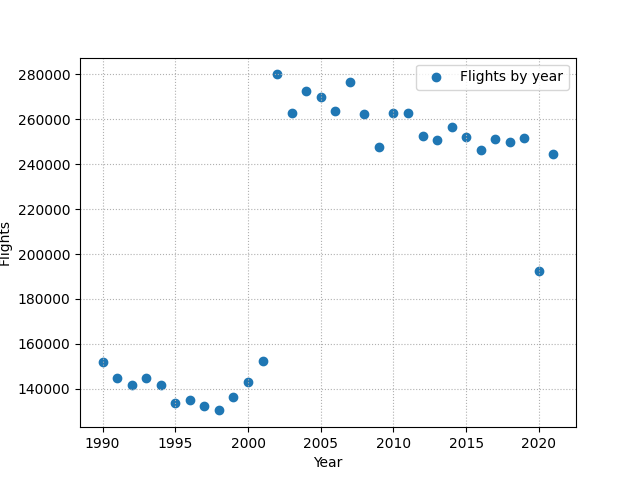
\includegraphics{./graphs/Count of flights} 

}

\caption{Trend of domestic flights in the USA}\label{fig:aviation-flights-image}
\end{figure}

\begin{table}[tbp]

\begin{center}
\begin{threeparttable}

\caption{\label{tab:aviation-jobs-schema}Trend of jobs in the aviation industry}

\begin{tabular}{lll}
\toprule
column & \multicolumn{1}{c}{Context} & \multicolumn{1}{c}{Datatype}\\
\midrule
ID & Unique identifier for each year & string\\
Year & Year for the statictic & date: yyyy\\
Period & Month of the statictic & date: mm\\
Label & Month and Year combined for label & string\\
Value & Year "1" acts as benchmark and subsequest year shows the & float\\
 & percent increase/decrease in employement numbers & \\
\bottomrule
\end{tabular}

\end{threeparttable}
\end{center}

\end{table}

\begin{table}[tbp]

\begin{center}
\begin{threeparttable}

\caption{\label{tab:aviation-incidents-schema}Trend of incidents in the aviation industry, scope limited to the USA}

\begin{tabular}{lll}
\toprule
column & \multicolumn{1}{c}{description} & \multicolumn{1}{c}{fieldtype}\\
\midrule
Data dimension & Data dimension from source & 168461 x 14\\
Scope limited data & Data dimension after limiting the scope USA & 151665 x 14\\
Duplicates removed & Data after removing duplicates & 80728 x 14\\
event id & Unique identifier for the event & string\\
ntsb number & Unique identifier created by the NTSB & string\\
event state & Name of the state where the event occured & string\\
event country & Country of the state where the event occured & string\\
event year & Year (timestamp) of the event & date: yyyy\\
event month & Month (timestamp) of the event & date: mm\\
fatal injuries on ground & Fatalities on ground of the event site & integer\\
minor injuries on ground & Minor injuries at the event site & integer\\
serious injuries on\ \ ground & Serious injuries at the event site & integer\\
total injuries on flight & Total injuries on flight & integer\\
minor injuries in flight & Fatal injuries on flight & integer\\
serious injuries in flight & Minor injuries on flight & integer\\
fatal injures in flight & Serious injuries on flight & integer\\
total ground injuries & Calculated Field: Total ground injuries & integer\\
total flight injuries & Calculated Field: Total flight injuries & integer\\
total injuries & Calculated Field: Total injuries & integer\\
\bottomrule
\end{tabular}

\end{threeparttable}
\end{center}

\end{table}

\begin{figure}

{\centering 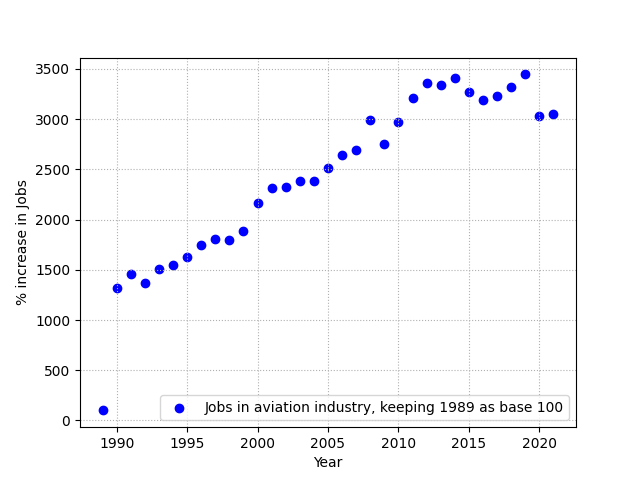
\includegraphics{./graphs/Jobs in the aviation industry} 

}

\caption{Trend of aviation jobs over the years}\label{fig:aviation-jobs-image}
\end{figure}

\begin{figure}

{\centering 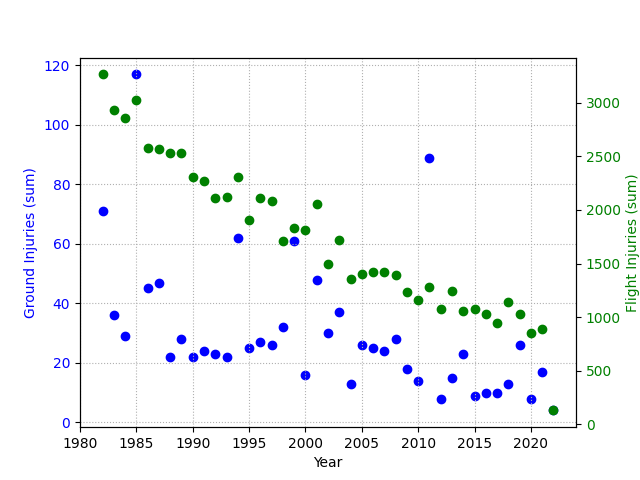
\includegraphics{./graphs/flight_injuries} 

}

\caption{Trend of injuries across time}\label{fig:aviation-incident-plot}
\end{figure}

The table \ref{tab:aviation-flights} is a scoped table used for the analysis. There are no \texttt{NULL} or \texttt{empty} values in the table and therefore do not need to be treated for it. Therefore, this data is derived from official sources and, therefore, not treated. To see the trend for the number of flights in the USA, refer to figure \ref{fig:aviation-flights-image}. A count of flights per year demonstrates the trend of aviation utilization, shown in figure \ref{fig:aviation-flights-image}\\

The flights in the domestic USA had a sudden rise around 2002. With a significant dip in the year 2020 on account of the global pandemic of COVID-19. The following year, the number of flights jumped back to its ``normal'' trend.

There are no \texttt{NULL} and \texttt{empty} entries in the dataset from the Blevins (2010). There were not any. Then the dataset is corrected to the expected format for analysis. Finally, a count of records for each year makes the figure (\textbf{ref?})(fig:aviation-flights-image).

\hypertarget{jobs-in-the-aviation-industry}{%
\subsubsection{Jobs in the aviation industry}\label{jobs-in-the-aviation-industry}}

To measure how automation has affected the aviation industry, we observe the jobs in the aviation industry. The Bureau of Labor Statistics Labor Statistics (2022) provides the data for this analysis. The table \ref{tab:aviation-jobs-schema} shows the data schema. There are no \texttt{NULL} or \texttt{empty} values in the data; hence cleanup is not required. Since this data comes directly from the Bureau of Labor Statistics and, therefore, is not scoped for outliers.\\

The data is grouped by year and then summed for each year. Modeling the dataset like this will show the trend for aviation jobs across the USA. From the trend, the number of jobs in the aviation industry seems to be increasing over the years, shown in figure \ref{fig:aviation-jobs-image}. There could be many reasons for this, including the rise of cheaper flight carriers, increased demand for flights, and increased connectivity requests from the population, among others.

\hypertarget{incidents-in-the-aviation-industry}{%
\subsubsection{Incidents in the aviation industry}\label{incidents-in-the-aviation-industry}}

A mandate for new safety standards follows a trend of similar incidents. New automation opportunity arises from these safety standards. Auto-pilot was introduced for long flights to relieve pilots from fatigue. Unpredictable climatic factors at the airports saw the introduction of automatic take-off and landing assistance. Overall the safety standards increase following incidents. Board (2022) provides us with the incident figures with the count of fatalities and injuries. Table \ref{tab:aviation-incidents-schema} describe the datasets schema.\\

The dataset contains \texttt{NULL} in the integer columns. \texttt{0} replaces the \texttt{NULL} records. \texttt{Total\ Ground\ Injures} and \texttt{Total\ Flight\ Injuries} are calculated columns to understand the trend of injuries across \texttt{year,} displayed in figure \ref{fig:aviation-incident-plot}\\

The plot shows the downward trend of injuries, both in flight and on the ground. The blue plots show the number of ground injuries over the years, and the green plots show the number of flight injuries. Figure \ref{fig:aviation-incident-plot} is a dual-axis graph to indicate the number of injuries from 1981 to 2021\\

\hypertarget{automobile-industry}{%
\subsection{Automobile Industry}\label{automobile-industry}}

\begin{table}[tbp]

\begin{center}
\begin{threeparttable}

\caption{\label{tab:car-safety-introduction}Vehicle Safety Standards}

\begin{tabular}{ll}
\toprule
Safety.Measure & \multicolumn{1}{c}{Year}\\
\midrule
4 wheel Hydraulic Breaks & 1922\\
Safety Glass & 1930\\
Seat Belts & 1930\\
Crash Test & 1934\\
Backup Break System & 1936\\
Flat \& Smooth Dashboard & 1937\\
Rounded Door Handled & 1937\\
Rubberised Wipers & 1937\\
Padded Read of Front Seat for Rear Passengers & 1937\\
Padded Dashboard & 1947\\
Front Steel Bulkhead \& Safety Chamber & 1947\\
Safety Cage & 1949\\
Standard Disk Breaks & 1949\\
Bumper Shocks & 1955\\
3-point safety belts & 1959\\
Elimination of protruding knobs & 1967\\
4-way Hazard Flashers & 1967\\
Uniform P-R-N-D-L gear sequence for automatic transmissions & 1967\\
Dual-circuit brake hydraulic system & 1967\\
Airbags & 1974\\
Central 3rd Break Light Mandate & 1986\\
Advanced Break Warning System & 1989\\
Anti Skid System & 2009\\
Minimum Crush Load Requirement Mandate & 2009\\
\bottomrule
\end{tabular}

\end{threeparttable}
\end{center}

\end{table}

\begin{table}[tbp]

\begin{center}
\begin{threeparttable}

\caption{\label{tab:car-registration-schema}Car Sales in the United States}

\begin{tabular}{lll}
\toprule
column & \multicolumn{1}{c}{Description} & \multicolumn{1}{c}{datatype}\\
\midrule
Year & Year of car sales & date: yyyy\\
Domestic Sales & Total cars sold in the US & float\\
\bottomrule
\end{tabular}

\end{threeparttable}
\end{center}

\end{table}

\begin{figure}

{\centering 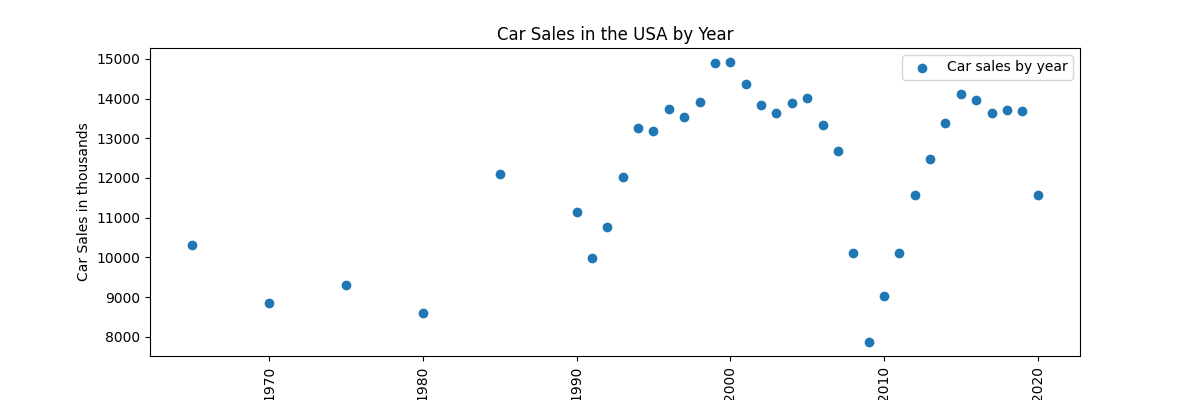
\includegraphics{./graphs/car_sales} 

}

\caption{Cars registered in the US}\label{fig:car-registered}
\end{figure}

\begin{table}[tbp]

\begin{center}
\begin{threeparttable}

\caption{\label{tab:car-accidents-schema}Automobile accidents in the United States by year}

\begin{tabular}{lll}
\toprule
column & \multicolumn{1}{c}{Description} & \multicolumn{1}{c}{datatype}\\
\midrule
ST\_CASE & Unique identifier for the car crash register & string\\
MONTH & Month of accident & date: mm\\
YEAR & Year of accident & date: yyyy\\
FATALS & Injuries and Fatalities & interger\\
\bottomrule
\end{tabular}

\end{threeparttable}
\end{center}

\end{table}

\begin{figure}

{\centering 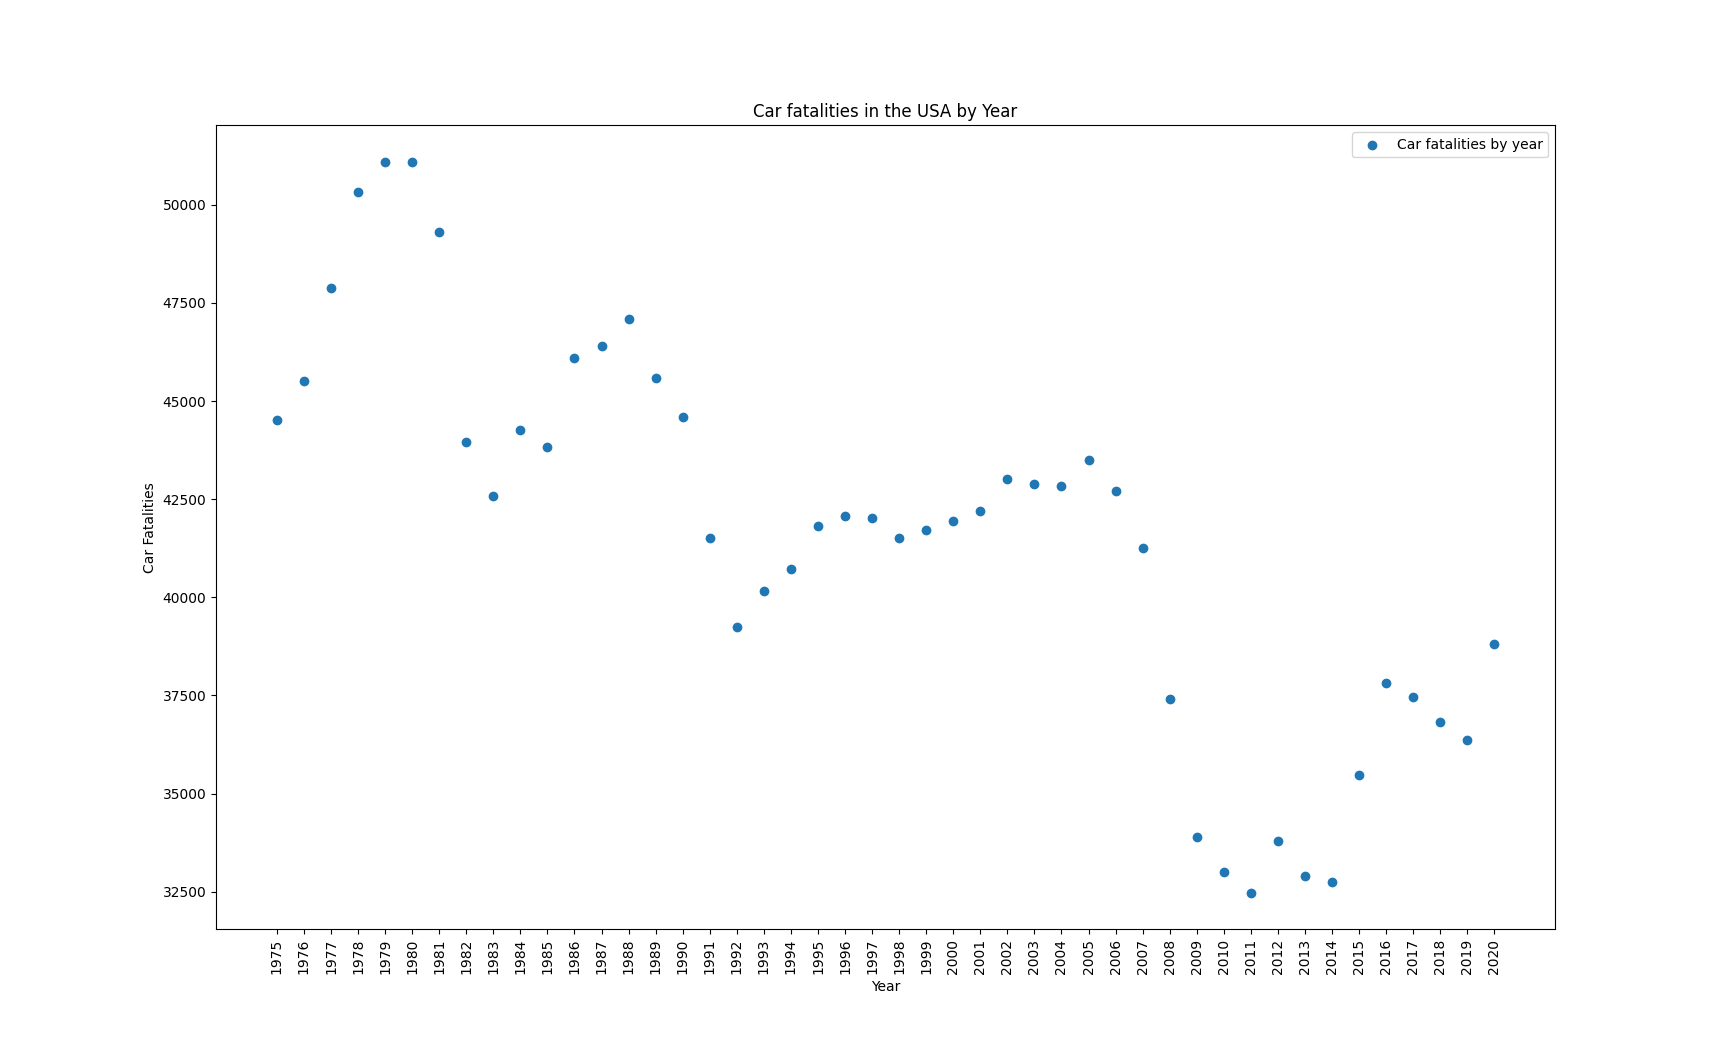
\includegraphics{./graphs/car_fatalities} 

}

\caption{Cars accidents in the US}\label{fig:car-incidents}
\end{figure}

\begin{table}[tbp]

\begin{center}
\begin{threeparttable}

\caption{\label{tab:tesla-deaths-schema}Data Schema for the deaths caused by Tesla automobiles}

\begin{tabular}{lll}
\toprule
column & \multicolumn{1}{c}{Description} & \multicolumn{1}{c}{datatypes}\\
\midrule
Year & Year of the incident & date: yyyy\\
Deaths & Deaths of humans involved in that incident & integer\\
Autopilot deaths & Deaths caused by autopilot system & integer\\
\bottomrule
\end{tabular}

\end{threeparttable}
\end{center}

\end{table}

\begin{figure}

{\centering 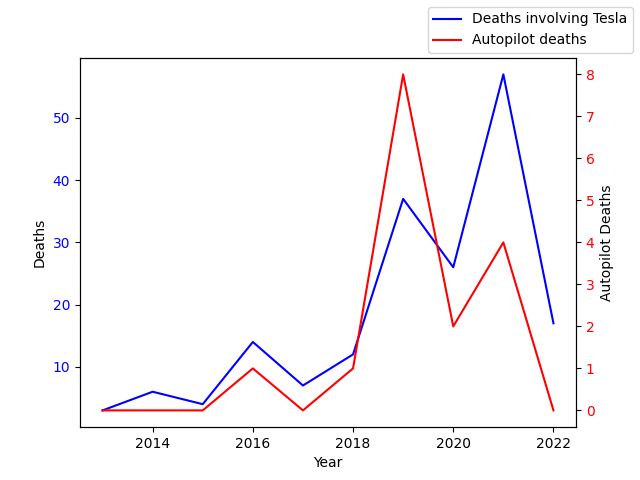
\includegraphics{./graphs/tesla_deaths} 

}

\caption{Time series of the deaths involving Tesla}\label{fig:tesla-deaths}
\end{figure}

From the authors' point of view, the motor vehicle industry is gaining on the levels of automation. Following the levels of automation defined by Administration (n.d.), the vehicles we drive have moved from level 0 to level 1 with adaptive cruise control systems. Then it jumped from level 1 to level 2, with corporations helping in the `highway pilot' system. The `Highway Pilot' system controls the steering and braking systems but still requires human control to signal the systems. At the time of writing, Tesla and Waymo are testing these systems. There are lessons to pick up from the aviation industry with a level 4 to level 5 system.\\

Motor vehicles, similar to aviation, have had many safety improvements. It is hard to picture a car without high-powered headlights and turn signals. A simple look at the Wikipedia page for automotive safety will list all the safety improvements and table \ref{tab:car-safety-introduction} does precisely that (2022), Straith (2022), Andréasson et al. (2000), Sparke (1999), Hudson (1936), Chrysler (1937), Plymouth (1937), Dodge (1940), Kimes and Austen (1996), (1948), Saab (1949), Flory (2008), Corporation (1955), Volvo (1959), Kashyap (2017), Popa (2009), Hard (2010). Fatalities dropped with the introduction of these safety standards.\\

\hypertarget{automobile-registered}{%
\subsubsection{Automobile Registered}\label{automobile-registered}}

Bureau of Transportation Statics provides us with the dataset of the commercial cars registered in the United States (B. of Transportation Statistics (2021)). The dataset is concise with the number of cars registered for that year. There are no \texttt{NULL} or \texttt{empty} rows in this dataset and therefore do not require any cleaning. Since the Bureau of Transportation Statistics maintains the data set with the Department of Transportation (B. of Transportation Statistics (2021)), data is considered accurate. The data is grouped by year from the source, and therefore the graph \ref{fig:car-registered} needs no processing. This graph is a direct plot of cars registered in the United States. The trend graph shows a noticeable drop in the global recession of 2008. Table \ref{tab:car-registration-schema} shows the schema of the data.\\

\hypertarget{automobile-incidents}{%
\subsubsection{Automobile Incidents}\label{automobile-incidents}}

The trend graph \ref{fig:car-incidents} shows the impact of introducing safety standards. National Highway Traffic Safety Administration (Administration (2016)) provides the dataset for automobile accidents over the years. The dataset does not contain \texttt{NULL} or \texttt{empty.} The federal government maintains this dataset; hence, it does not need to scope for outliers. Table \ref{tab:car-accidents-schema} references the data schema. The dataset contains multiple columns. The table \ref{tab:car-accidents-schema} shows the scope of the dataset needed for this analysis. The data graph is created by aggregating the \texttt{FATALS} column on \texttt{YEAR.}

\hypertarget{self-driving-automobile-incidents}{%
\subsubsection{Self Driving Automobile Incidents}\label{self-driving-automobile-incidents}}

The automobile industry is trending toward the driverless standard. Therefore, it is imperative to analyze the incidents involving self-driving cars. At the time of this research, Tesla's involved in 254 deaths on the road. Of these 254 deaths, 24 are caused by Tesla's Autopilot system (Deaths (2022)), with 16 in the USA. Tesla's first car was released in 2008, and the autopilot was introduced in 2013 Reed (2020). These deaths are significantly less than the national average, constituting less than 0.0001\% of the whole. The table \ref{tab:tesla-deaths-schema} shows the data schema in scope for this analysis. Figure \ref{fig:tesla-deaths} shows the time-series graph involving tesla cars with and without an autopilot system.

\hypertarget{results}{%
\section{Results}\label{results}}

Aviation, considered a level 4 automation, shows a negligible impact on employment. Moreover, forgiving the dip caused by the global pandemic of COVID-19, the trend is positive. Therefore, concluding that the impact of automation has not resulted in employment loss. Now, consider the safety metric. The number of flights by major airlines in the domestic US has normalized. The incidents, however, are on a sharp downward trend. Incidents include both ground and in-flight accidents. Hence, the conclusion, automation for safety standards save lives. Therefore, there is no significant evidence for our hypothesis to be true from the analysis results.\\

We see similar trends in extending our understanding of the aviation industry and projecting it to the automobile industry, primarily focusing on safety, as there is no automation in the commercial section of the automation to draw any analysis. Over the years of including safety standards in the consumer automobile, the fatality numbers are on a negative trend. However, there has been an increase in the past decade. The positive trend correlates with the increase in the number of cars on the road. Similarly, there is a seasonality of fatalities observed over the years. For every increasing trend, a new automative system is introduced to make the roads safer. This trend seems to follow the onslaught of self-driving cars. The consumer section will bring changes in the commercial section as well. Therefore, making the stage for self-driving cars a highly likely event.

\hypertarget{discussion}{%
\section{Discussion}\label{discussion}}

\hypertarget{result-summary}{%
\subsection{Result Summary}\label{result-summary}}

It seems highly likely that the lessons from the aviation industry can be extrapolated to the automobile industry. A new safety standard will be introduced, giving way to self-driving and potentially driverless cars for all consumer vehicles shortly. Therefore, making a case for a level 5 automation is highly likely in the coming decades.\\

\hypertarget{limitations}{%
\subsection{Limitations}\label{limitations}}

There are some limitations to this analysis:
1. An in-depth analysis is warranted for a more decisive result in every section. Each point increase or decrease in the trend needs investigation. Similarly, seasonality in the results has to be studied in-breath and compared with global findings.
2. Only the United States of America is in scope for this analysis. A European market analysis could add some supporting evidence.
3. The trend results from America and Europe can be compared with the developing markets to correlate with the global trend.\\
Extending this research to other industrial sectors can support or contradict this analysis. The financial and manufacturing industries can enrich this research with more points.

\newpage

\hypertarget{references}{%
\section{References}\label{references}}

\begingroup
\setlength{\parindent}{-0.5in}
\setlength{\leftskip}{0.5in}

\hypertarget{refs}{}
\begin{CSLReferences}{1}{0}
\leavevmode\vadjust pre{\hypertarget{ref-abernathy1975technology}{}}%
Abernathy, W. J., \& Townsend, P. L. (1975). Technology, productivity and process change. \emph{Technological Forecasting and Social Change}, \emph{7}(4), 379--396.

\leavevmode\vadjust pre{\hypertarget{ref-acemoglu2011skills}{}}%
Acemoglu, D., \& Autor, D. (2011). Skills, tasks and technologies: Implications for employment and earnings. In \emph{Handbook of labor economics} (Vol. 4, pp. 1043--1171). Elsevier.

\leavevmode\vadjust pre{\hypertarget{ref-levelsofautomation}{}}%
Administration, N. H. T. S. (n.d.). \emph{The evolution of automated safety technologies}. US Department of Transportation. \url{https://www.nhtsa.gov/technology-innovation/automated-vehicles-safety}

\leavevmode\vadjust pre{\hypertarget{ref-anonymous_2016_nhtsa}{}}%
Administration, N. H. T. S. (2016). \emph{NHTSA}. NHTSA; Department of Transportation. \url{https://www.nhtsa.gov/research-data/fatality-analysis-reporting-system-fars}

\leavevmode\vadjust pre{\hypertarget{ref-runeandrasson_2000_the}{}}%
Andréasson, R., Bäckström, C.-G., \& Kulturvardskommittén, Vattenfall. (2000). \emph{The seat belt : Swedish research and development for global automotive safety.} Eo Print.

\leavevmode\vadjust pre{\hypertarget{ref-R-papaja}{}}%
Aust, F., \& Barth, M. (2022). \emph{{papaja}: {Prepare} reproducible {APA} journal articles with {R Markdown}}. \url{https://github.com/crsh/papaja}

\leavevmode\vadjust pre{\hypertarget{ref-autor2003skill}{}}%
Autor, D. H., Levy, F., \& Murnane, R. J. (2003). The skill content of recent technological change: An empirical exploration. \emph{The Quarterly Journal of Economics}, \emph{118}(4), 1279--1333.

\leavevmode\vadjust pre{\hypertarget{ref-badue2021self}{}}%
Badue, C., Guidolini, R., Carneiro, R. V., Azevedo, P., Cardoso, V. B., Forechi, A., Jesus, L., Berriel, R., Paixao, T. M., Mutz, F.others. (2021). Self-driving cars: A survey. \emph{Expert Systems with Applications}, \emph{165}, 113816.

\leavevmode\vadjust pre{\hypertarget{ref-bainbridge1982ironies}{}}%
Bainbridge, L. (1982). Ironies of automation. \emph{IFAC Proceedings Volumes}, \emph{15}(6), 129--135.

\leavevmode\vadjust pre{\hypertarget{ref-rhbarbhayagit}{}}%
Barbhaya, G. R. (2022). \emph{Safety and jobs in automated world}. \url{https://github.com/rhbarbhaya/Safety-and-Jobs-in-Automated-World}

\leavevmode\vadjust pre{\hypertarget{ref-berberian2012automation}{}}%
Berberian, B., Sarrazin, J.-C., Le Blaye, P., \& Haggard, P. (2012). Automation technology and sense of control: A window on human agency. \emph{PloS One}, \emph{7}(3), e34075.

\leavevmode\vadjust pre{\hypertarget{ref-beresnevicius_2019}{}}%
Beresnevicius, R. (2019). Automation in the aviation industry - the future is automated. In \emph{AeroTime Hub}. AeroTime Hub. \url{https://www.aerotime.aero/articles/23162-automation-aviation-industry}

\leavevmode\vadjust pre{\hypertarget{ref-AirlineI37}{}}%
Blevins, J. (2010). \emph{Airline industry datasets}. \url{https://jblevins.org/notes/airline-data}.

\leavevmode\vadjust pre{\hypertarget{ref-Accident29}{}}%
Board, N. T. S. (2022). \emph{Accident data}. \url{https://www.ntsb.gov/safety/data/Pages/Data_Stats.aspx}.

\leavevmode\vadjust pre{\hypertarget{ref-chrysler_1937_directory}{}}%
Chrysler. (1937). \emph{Directory index: Chrysler\_and\_imperial/1937\_chrysler/1937\_chrysler\_brochure}. Oldcarbrochures.com. \url{http://www.oldcarbrochures.com/static/NA/Chrysler_and_Imperial/1937_Chrysler/1937_Chrysler_Brochure/1937\%20Chrysler-08-09.html}

\leavevmode\vadjust pre{\hypertarget{ref-corporation_1955_popular}{}}%
Corporation, B. (1955). \emph{Popular science}. Google Books; Bonnier Corporation. \url{https://books.google.com/books?id=biYDAAAAMBAJ\&pg=-PA27\&dq=popular+science+1930\&hl=en\&sa=X\&ei=I5ICT8KZKsvlgge97s22Ag\&ved=0CEsQ6AEwBjhu\#v=onepage\&q\&f=true}

\leavevmode\vadjust pre{\hypertarget{ref-daily2017self}{}}%
Daily, M., Medasani, S., Behringer, R., \& Trivedi, M. (2017). Self-driving cars. \emph{Computer}, \emph{50}(12), 18--23.

\leavevmode\vadjust pre{\hypertarget{ref-davenport2019potential}{}}%
Davenport, T., \& Kalakota, R. (2019). The potential for artificial intelligence in healthcare. \emph{Future Healthcare Journal}, \emph{6}(2), 94.

\leavevmode\vadjust pre{\hypertarget{ref-tesladeaths_2022_tesladeathscom}{}}%
Deaths, T. (2022). \emph{TeslaDeaths.com: Digital record of tesla crashes resulting in death}. TeslaDeaths.com. \url{https://www.tesladeaths.com}

\leavevmode\vadjust pre{\hypertarget{ref-dodge_1940_directory}{}}%
Dodge. (1940). \emph{Directory index: Dodge/1940\_dodge/1940\_dodge\_brochure}. Oldcarbrochures.com. \url{http://www.oldcarbrochures.com/static/NA/Dodge/1940_Dodge/1940_Dodge_Brochure/1940\%20Dodge-09-10.html}

\leavevmode\vadjust pre{\hypertarget{ref-_2022_directory}{}}%
Duesenberg. (2022). \emph{Directory index: Duesenberg/1922\_duesenberg\_model\_a\_catalogue}. Oldcarbrochures.com. \url{http://www.oldcarbrochures.com/static/NA/Duesenberg/1922_Duesenberg_Model_A_Catalogue/1922\%20Duesenberg\%20Model\%20A\%20Catalogue-06.html}

\leavevmode\vadjust pre{\hypertarget{ref-evangelista2012impact}{}}%
Evangelista, R., \& Vezzani, A. (2012). The impact of technological and organizational innovations on employment in european firms. \emph{Industrial and Corporate Change}, \emph{21}(4), 871--899.

\leavevmode\vadjust pre{\hypertarget{ref-fleming2020short}{}}%
Fleming, S. (2020). \emph{A short history of jobs and automation}.

\leavevmode\vadjust pre{\hypertarget{ref-jkellyflory_2008_american}{}}%
Flory, J. K. (2008). \emph{American cars, 1946-1959 : Every model, year by year}. Mcfarland \& Co.

\leavevmode\vadjust pre{\hypertarget{ref-hard_2010_nhtsa}{}}%
Hard, G. (2010). \emph{NHTSA declines to revisit roof-crush standard}. www.consumerreports.org; Consumer Reports. \url{https://www.consumerreports.org/cro/news/2010/04/nhtsa-declines-to-revisit-roof-crush-standard/index.htm}

\leavevmode\vadjust pre{\hypertarget{ref-hills1989william}{}}%
Hills, R. L. (1989). William lee and his knitting machine. \emph{Journal of the Textile Institute}, \emph{80}(2), 169--184.

\leavevmode\vadjust pre{\hypertarget{ref-hudson_1936_directory}{}}%
Hudson. (1936). \emph{Directory index: Hudson/1936\_hudson/1936\_hudson\_-\_how\_what\_why}. Oldcarbrochures.com. \url{http://www.oldcarbrochures.com/static/NA/Hudson/1936_Hudson/1936_Hudson_-_How_What_Why/1936\%20Hudsons\%20HWW-089\%20001.html}

\leavevmode\vadjust pre{\hypertarget{ref-jamsa2007future}{}}%
Jämsä-Jounela, S.-L. (2007). Future trends in process automation. \emph{Annual Reviews in Control}, \emph{31}(2), 211--220.

\leavevmode\vadjust pre{\hypertarget{ref-kashyap_2017_safety}{}}%
Kashyap, D. P. (2017). Safety and security in automobile and its history. \emph{International Journal of Creative Research Thoughts}, \emph{5}, 965. \url{https://www.ijcrt.org/papers/IJCRT1801132.pdf}

\leavevmode\vadjust pre{\hypertarget{ref-beverlyraekimes_1996_standard}{}}%
Kimes, B. R., \& Austen, H. (1996). \emph{Standard catalog of american cars : 1805-1942}. Krause Publications.

\leavevmode\vadjust pre{\hypertarget{ref-BLSDataV82}{}}%
Labor Statistics, U. S. B. of. (2022). \emph{BLS data viewer}. \url{https://beta.bls.gov/dataViewer/view/timeseries/PCU481---481---}.

\leavevmode\vadjust pre{\hypertarget{ref-lala2020autonomous}{}}%
Lala, J. H., Landwehr, C. E., \& Meyer, J. F. (2020). Autonomous vehicle safety: Lessons from aviation. \emph{Communications of the ACM}, \emph{63}(9), 28--31.

\leavevmode\vadjust pre{\hypertarget{ref-mackie_2021}{}}%
Mackie, C. (2021). Beware professional services workers: Robots are coming for your job too! In \emph{Forbes}. Forbes Magazine. \url{https://www.forbes.com/sites/calvinmackie/2021/09/30/beware-professional-services-workers-robots-are-coming-for-your-job-too/?sh=2fd2aa5b5237}

\leavevmode\vadjust pre{\hypertarget{ref-mahmud2020robotics}{}}%
Mahmud, M. S. A., Abidin, M. S. Z., Emmanuel, A. A., \& Hasan, H. S. (2020). Robotics and automation in agriculture: Present and future applications. \emph{Applications of Modelling and Simulation}, \emph{4}, 130--140.

\leavevmode\vadjust pre{\hypertarget{ref-mcclure2018you}{}}%
McClure, P. K. (2018). {``You're fired,''} says the robot: The rise of automation in the workplace, technophobes, and fears of unemployment. \emph{Social Science Computer Review}, \emph{36}(2), 139--156.

\leavevmode\vadjust pre{\hypertarget{ref-mohanraj2016field}{}}%
Mohanraj, I., Ashokumar, K., \& Naren, J. (2016). Field monitoring and automation using IOT in agriculture domain. \emph{Procedia Computer Science}, \emph{93}, 931--939.

\leavevmode\vadjust pre{\hypertarget{ref-nie2001internet}{}}%
Nie, N., \& Erbring, L. (2001). \emph{Internet and society: A preliminary report. The digital divide: Facing a crisis or creating a myth}. Cambridge: MIT Press.

\leavevmode\vadjust pre{\hypertarget{ref-peleska1996test}{}}%
Peleska, J., \& Siegel, M. (1996). \emph{Test automation of safety-critical reactive systems}.

\leavevmode\vadjust pre{\hypertarget{ref-plymouth_1937_directory}{}}%
Plymouth. (1937). \emph{Directory index: Plymouth/1937\_plymouth/1937\_plymouth\_biggest\_value\_brochure}. Oldcarbrochures.com. \url{http://www.oldcarbrochures.com/static/NA/Plymouth/1937_Plymouth/1937_Plymouth_Biggest_Value_Brochure/1937\%20Plymouth\%20Biggest\%20Value-19.html}

\leavevmode\vadjust pre{\hypertarget{ref-popa_2009_citroen}{}}%
Popa, B. (2009). \emph{Citroen C5 with snow motion intelligent anti-skid system}. autoevolution; autoevolution. \url{https://www.autoevolution.com/news/citroen-c5-with-snow-motion-intelligent-anti-skid-system-4542.html}

\leavevmode\vadjust pre{\hypertarget{ref-python.org_2021}{}}%
Python release python 3.9.7. (2021). In \emph{Python.org}. \url{https://www.python.org/downloads/release/python-397/}

\leavevmode\vadjust pre{\hypertarget{ref-reed_2020_history}{}}%
Reed, E. (2020). \emph{History of tesla: Timeline and facts}. TheStreet; TheStreet. \url{https://www.thestreet.com/technology/history-of-tesla-15088992}

\leavevmode\vadjust pre{\hypertarget{ref-rice2019driverless}{}}%
Rice, D. (2019). The driverless car and the legal system: Hopes and fears as the courts, regulatory agencies, waymo, tesla, and uber deal with this exciting and terrifying new technology. \emph{Journal of Strategic Innovation and Sustainability}, \emph{14}(1), 134--146.

\leavevmode\vadjust pre{\hypertarget{ref-robinson2003new}{}}%
Robinson, J. P., DiMaggio, P., \& Hargittai, E. (2003). New social survey perspectives on the digital divide. \emph{It \& Society}, \emph{1}(5), 1--22.

\leavevmode\vadjust pre{\hypertarget{ref-saab_1949_saab}{}}%
Saab. (1949). \emph{Saab shows its first concept car - latest car news from 4Car}. web.archive.org. \url{https://web.archive.org/web/20080519035733/http://www.channel4.com/4car/news/news-story.jsp?news_id=6034}

\leavevmode\vadjust pre{\hypertarget{ref-sarangi2016automation}{}}%
Sarangi, S., Umadikar, J., \& Kar, S. (2016). Automation of agriculture support systems using wisekar: Case study of a crop-disease advisory service. \emph{Computers and Electronics in Agriculture}, \emph{122}, 200--210.

\leavevmode\vadjust pre{\hypertarget{ref-schwall2020waymo}{}}%
Schwall, M., Daniel, T., Victor, T., Favaro, F., \& Hohnhold, H. (2020). Waymo public road safety performance data. \emph{arXiv Preprint arXiv:2011.00038}.

\leavevmode\vadjust pre{\hypertarget{ref-smith_2019}{}}%
Smith, A. (2019). Methodology. In \emph{Pew Research Center: Internet, Science \&amp; Tech}. Pew Research Center. \url{https://www.pewresearch.org/internet/2016/03/10/future-of-workforce-automation-methodology/}

\leavevmode\vadjust pre{\hypertarget{ref-song2003being}{}}%
Song, F. W. (2003). Being left behind: The discourse of fear in technological change. \emph{The Hedgehog Review}, \emph{5}(3), 26--43.

\leavevmode\vadjust pre{\hypertarget{ref-sparke_1999_wayback}{}}%
Sparke, L. J. (1999). \emph{Wayback machine}. web.archive.org. \url{https://web.archive.org/web/20071008232829/http://www.aesvn.org/resources/new-car-safety.pdf}

\leavevmode\vadjust pre{\hypertarget{ref-stanton1996fly}{}}%
Stanton, N. A., \& Marsden, P. (1996). From fly-by-wire to drive-by-wire: Safety implications of automation in vehicles. \emph{Safety Science}, \emph{24}(1), 35--49.

\leavevmode\vadjust pre{\hypertarget{ref-straith_2022_history}{}}%
Straith, C. L. (2022). \emph{History of straith clinic}. Straith Clinic; Straith Clinic. \url{https://straithclinic.com/history-of-straith-plastic-surgery-clinic-detroit.html}

\leavevmode\vadjust pre{\hypertarget{ref-strawn2016automation}{}}%
Strawn, G. (2016). Automation and future unemployment. \emph{IT Professional}, \emph{18}(1), 62--64.

\leavevmode\vadjust pre{\hypertarget{ref-R-base}{}}%
The r project for statistical computing. (2022). In \emph{The Comprehensive R Archive Network}. \url{https://cran.case.edu/}

\leavevmode\vadjust pre{\hypertarget{ref-thomis1972luddites}{}}%
Thomis, M. I. (1972). \emph{The luddites; machine-breaking in regency england}. Schocken Books Incorporated.

\leavevmode\vadjust pre{\hypertarget{ref-bureauoftransportationstatistics_2021_annual}{}}%
Transportation Statistics, B. of. (2021). \emph{Annual u.s. Motor vehicle production and domestic sales \textbar{} bureau of transportation statistics}. Bureau of Transportation Statistics; Department of Transportation. \url{https://www.bts.gov/content/annual-us-motor-vehicle-production-and-factory-wholesale-sales-thousands-units}

\leavevmode\vadjust pre{\hypertarget{ref-btstransstats}{}}%
Transportation Statistics, D. of. (2022). \emph{TranStats}. \url{https://transtats.bts.gov/DL_SelectFields.aspx?gnoyr_VQ=FIL\&QO_fu146_anzr=Nv4\%20Pn44vr45}.

\leavevmode\vadjust pre{\hypertarget{ref-_1948_directory}{}}%
Tucker. (1948). \emph{Directory index: Tucker/album/album}. web.archive.org. \url{https://web.archive.org/web/20101204091038/http://www.oldcarbrochures.com/static/NA/Tucker/album/album/1948\%20Tucker-04.html}

\leavevmode\vadjust pre{\hypertarget{ref-volvo_1959_safety}{}}%
Volvo. (1959). \emph{Safety innovation in cars \textbar{} volvo cars}. web.archive.org. \url{https://web.archive.org/web/20161113114437/http://www.volvocars.com/intl/about/our-company/heritage/innovations}

\leavevmode\vadjust pre{\hypertarget{ref-ward2000automation}{}}%
Ward, N. J. (2000). Automation of task processes: An example of intelligent transportation systems. \emph{Human Factors and Ergonomics in Manufacturing \& Service Industries}, \emph{10}(4), 395--408.

\end{CSLReferences}

\endgroup


\clearpage
\renewcommand{\listfigurename}{Figure captions}

\clearpage
\renewcommand{\listtablename}{Table captions}


\end{document}
